%% Lab Report for EEET2493_labreport_template.tex
%% V1.0
%% 2019/01/16
%% This is the template for a Lab report following an IEEE paper. Modified by Francisco Tovar after Michael Sheel original document.


%% This is a skeleton file demonstrating the use of IEEEtran.cls
%% (requires IEEEtran.cls version 1.8b or later) with an IEEE
%% journal paper.
%%
%% Support sites:
%% http://www.michaelshell.org/tex/ieeetran/
%% http://www.ctan.org/pkg/ieeetran
%% and
%% http://www.ieee.org/

%%*************************************************************************
%% Legal Notice:
%% This code is offered as-is without any warranty either expressed or
%% implied; without even the implied warranty of MERCHANTABILITY or
%% FITNESS FOR A PARTICULAR PURPOSE! 
%% User assumes all risk.
%% In no event shall the IEEE or any contributor to this code be liable for
%% any damages or losses, including, but not limited to, incidental,
%% consequential, or any other damages, resulting from the use or misuse
%% of any information contained here.
%%
%% All comments are the opinions of their respective authors and are not
%% necessarily endorsed by the IEEE.
%%
%% This work is distributed under the LaTeX Project Public License (LPPL)
%% ( http://www.latex-project.org/ ) version 1.3, and may be freely used,
%% distributed and modified. A copy of the LPPL, version 1.3, is included
%% in the base LaTeX documentation of all distributions of LaTeX released
%% 2003/12/01 or later.
%% Retain all contribution notices and credits.
%% ** Modified files should be clearly indicated as such, including  **
%% ** renaming them and changing author support contact information. **
%%*************************************************************************

\documentclass[journal]{IEEEtran}

%%%%%%%%%%%%%%%%%%%%%%%%%%%%%%%%%%%%%%%%%%%%%%%%%%%%%%%%%%%%%%

\usepackage[italian]{babel}

% *** CITATION PACKAGES ***
\usepackage[style=ieee]{biblatex} 
\bibliography{digital.bib}    %your file created using JabRef
\usepackage{hyperref}

% *** MATH PACKAGES ***
\usepackage{amsmath}
 \usepackage{multirow}

% *** PDF, URL AND HYPERLINK PACKAGES ***
\usepackage{url}
% correct bad hyphenation here
\hyphenation{op-tical net-works semi-conduc-tor}
\usepackage{graphicx}  %needed to include png, eps figures
\usepackage{float}  % used to fix location of images i.e.\begin{figure}[H]

\usepackage{csquotes} % correzione errore compilazione

%%%%%%%%%%%%%%%%%%%%%%%%%%%%%%%%%%%%%%%%%%%%%%%%%%%%%%%%%%%%%


\begin{document}

% paper title
\title{Laboratorio di elettronica digitale\\ 
%\small{1 gennaio 2020}
}

% author names 
\author{\begin{center}Matteo Barbagiovanni\textsuperscript{1},
        Stefano Barbero\textsuperscript{2},
        Federico Malnati\textsuperscript{3},
        Valerio Pagliarino\textsuperscript{4},
        {\small \\
        \textsuperscript{1}
        matteo.barbagiovanni@edu.unito.it -
        \textsuperscript{2}
        stefano.barbero376@edu.unito.it
        \textsuperscript{3}
        federico.malnati@edu.unito.it -
        \textsuperscript{4}
        valerio.pagliarino@edu.unito.it}
        \end{center}}% <-this % stops a space
        
% The report headers
\markboth{Università degli Studi di Torino - C.d.L. Triennale in Fisica - 10/11/21 - A.A. 2021-2022    \quad   \quad \quad \quad   \quad \quad \quad  \quad   \quad \quad \quad   \quad \quad LABORATORIO DI ELETTRONICA \quad \quad }%do not delete next lines
{Shell \MakeLowercase{\textit{et al.}}: Bare Demo of IEEEtran.cls for IEEE Journals}

% make the title area
\maketitle


%%%%%%%%%%%%%%%%%%%%%%%%%%%%%%%%%%%%%%%%%%%%%%%%%%%%%%%%%%%%%
%% Introduzione 
%%%%%%%%%%%%%%%%%%%%%%%%%%%%%%%%%%%%%%%%%%%%%%%%%%%%%%%%%%%%%

\begin{abstract} 
Introduzione all'esperienza
\end{abstract}

%%%%%%%%%%%%%%%%%%%%%%%%%%%%%%%%%%%%%%%%%%%%%%%%%%%%%%%%%%%%%
%%%%%%%%%%%%%%%%%%%%%%%%%%%%%%%%%%%%%%%%%%%%%%%%%%%%%%%%%%%%%

\section{Strumenti utilizzati}

\subsection{\textbf{Oscilloscopio Tektronix TBS1104}}

\begin{figure}[h!]
  \centering
  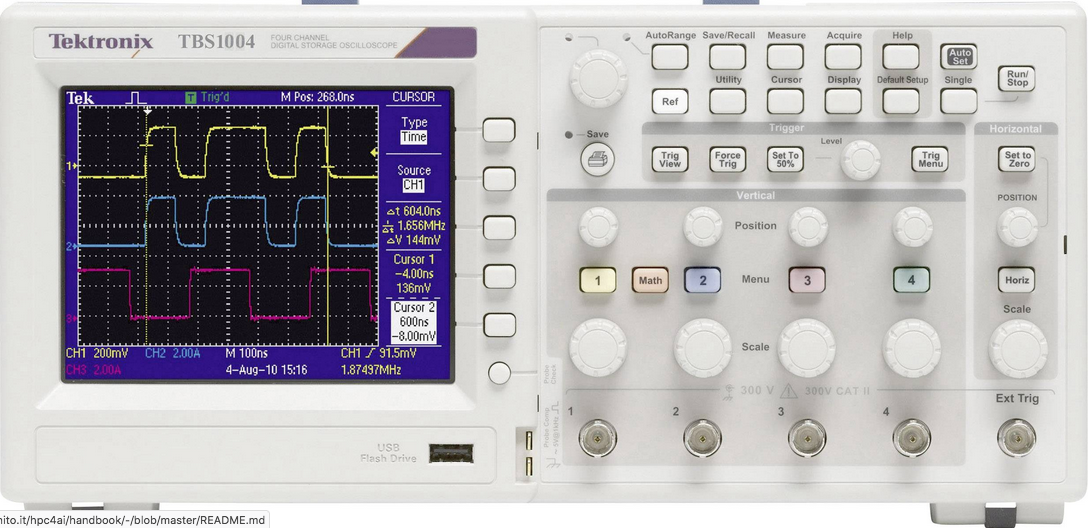
\includegraphics[width=0.18\textwidth]{lab-reports/Schematics-and-graphics/TEK Osc.png}
\end{figure}

La maggior parte delle misure di tensione e tempo è stata realizzata con un \textit{digital storage oscilloscope (DSO)} Tektronix 1104 con banda passante di 70 MHz, frequenza di campionamento massima di 1 GSa/s che consente fino a 5 ns/div di risoluzione temporale, 4 canali e 2.5K punti di memoria per finestra di acquisizione, risoluzione verticale di 8 bit e sensibilità fino a 10 mV/div.
\cite{A}

%%%%%%%%%%%%%%%%%%%%%%%%%%%%%%%%%%%%%%%%%%%%%%%%%%%%%%%%%%%%%

\subsection{\textbf{Generatore di funzioni Rigol DG1022Z}}

\begin{figure}[h!]
  \centering
  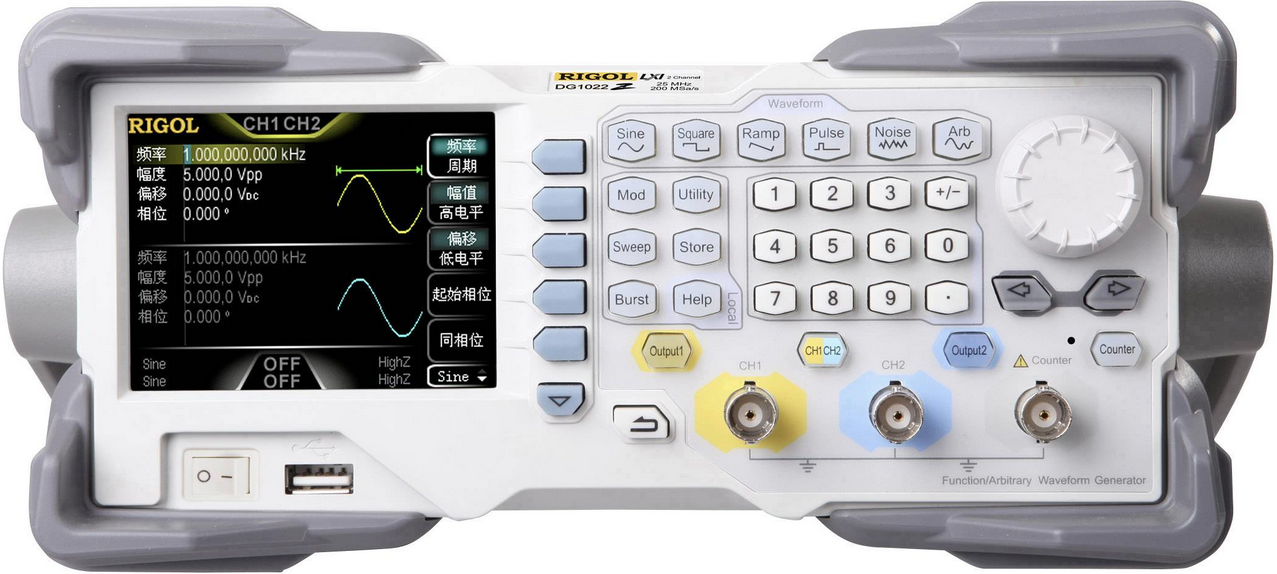
\includegraphics[width=0.18\textwidth]{lab-reports/Schematics-and-graphics/RIGOL Gen.png}
\end{figure}

Questo generatore di segnali arbitrari basato sulla sintesi digitale diretta (DDS) è stato impiegato per il pilotaggio dei circuiti. Il generatore ha una banda passante massima di 25 MHz, una frequenza di campionamento del DAC di 100 MSa/s e una risoluzione verticale di 14 bit. 
\cite{B}

%%%%%%%%%%%%%%%%%%%%%%%%%%%%%%%%%%%%%%%%%%%%%%%%%%%%%%%%%%%%%

\subsection{\textbf{Multimetro digitale Meterman 35XP e alimentatore da banco duale GW-Instek GPS-4303}}
Il corredo di strumentazione è stato completato con multimetro digitale Meterman 35XP utilizzato per misurare tensioni, resistenze e capacità, soprattutto in fase montaggio e verifica dei circuiti e da un generatore di tensione GW-Instek GPS-4303 con 4 canali a tensione e corrente variabile utilizzabili per fornire alimentazione duale all'amplificatore operazionale impiegato. La tensione proveniente da questo alimentatore è risultato in alcuni casi un po' rumorosa, pertanto sono stati aggiunti sulla breadboard dei condensatori livellanti in parallelo con valori nominali di $\sim$ 22 nF e $\sim$ 100 nF. Il multimetro ha una risoluzione di 3+3/4 cifre, un'accuratezza nelle misure di tensione DC di 0.5 \% della lettura + 1 * ultima cifra fino a 1KV e un'accuratezza nelle misure di resistenza di 1.0 \% della lettura + 4 * ultima cifra fino a 40 M$\Omega$. Per l'accuratezza nelle misure di capacità si rimanda al datasheet. L'alimentatore è invece in grado di fornire sui canali utilizzati fino a 30V / 5A. \cite{C} \cite{C}.


%%%%%%%%%%%%%%%%%%%%%%%%%%%%%%%%%%%%%%%%%%%%%%%%%%%%%%%%%%%%%%%%%%%%%%%%%%%%%%%%%%%%%%%%%%%%%%%%%%%%%%%%%%%%%%%%%%%%%%%%%%%%%%

\section{Il circuito completo}

\begin{figure*}[t]%[t]
\centering
\begin{center}
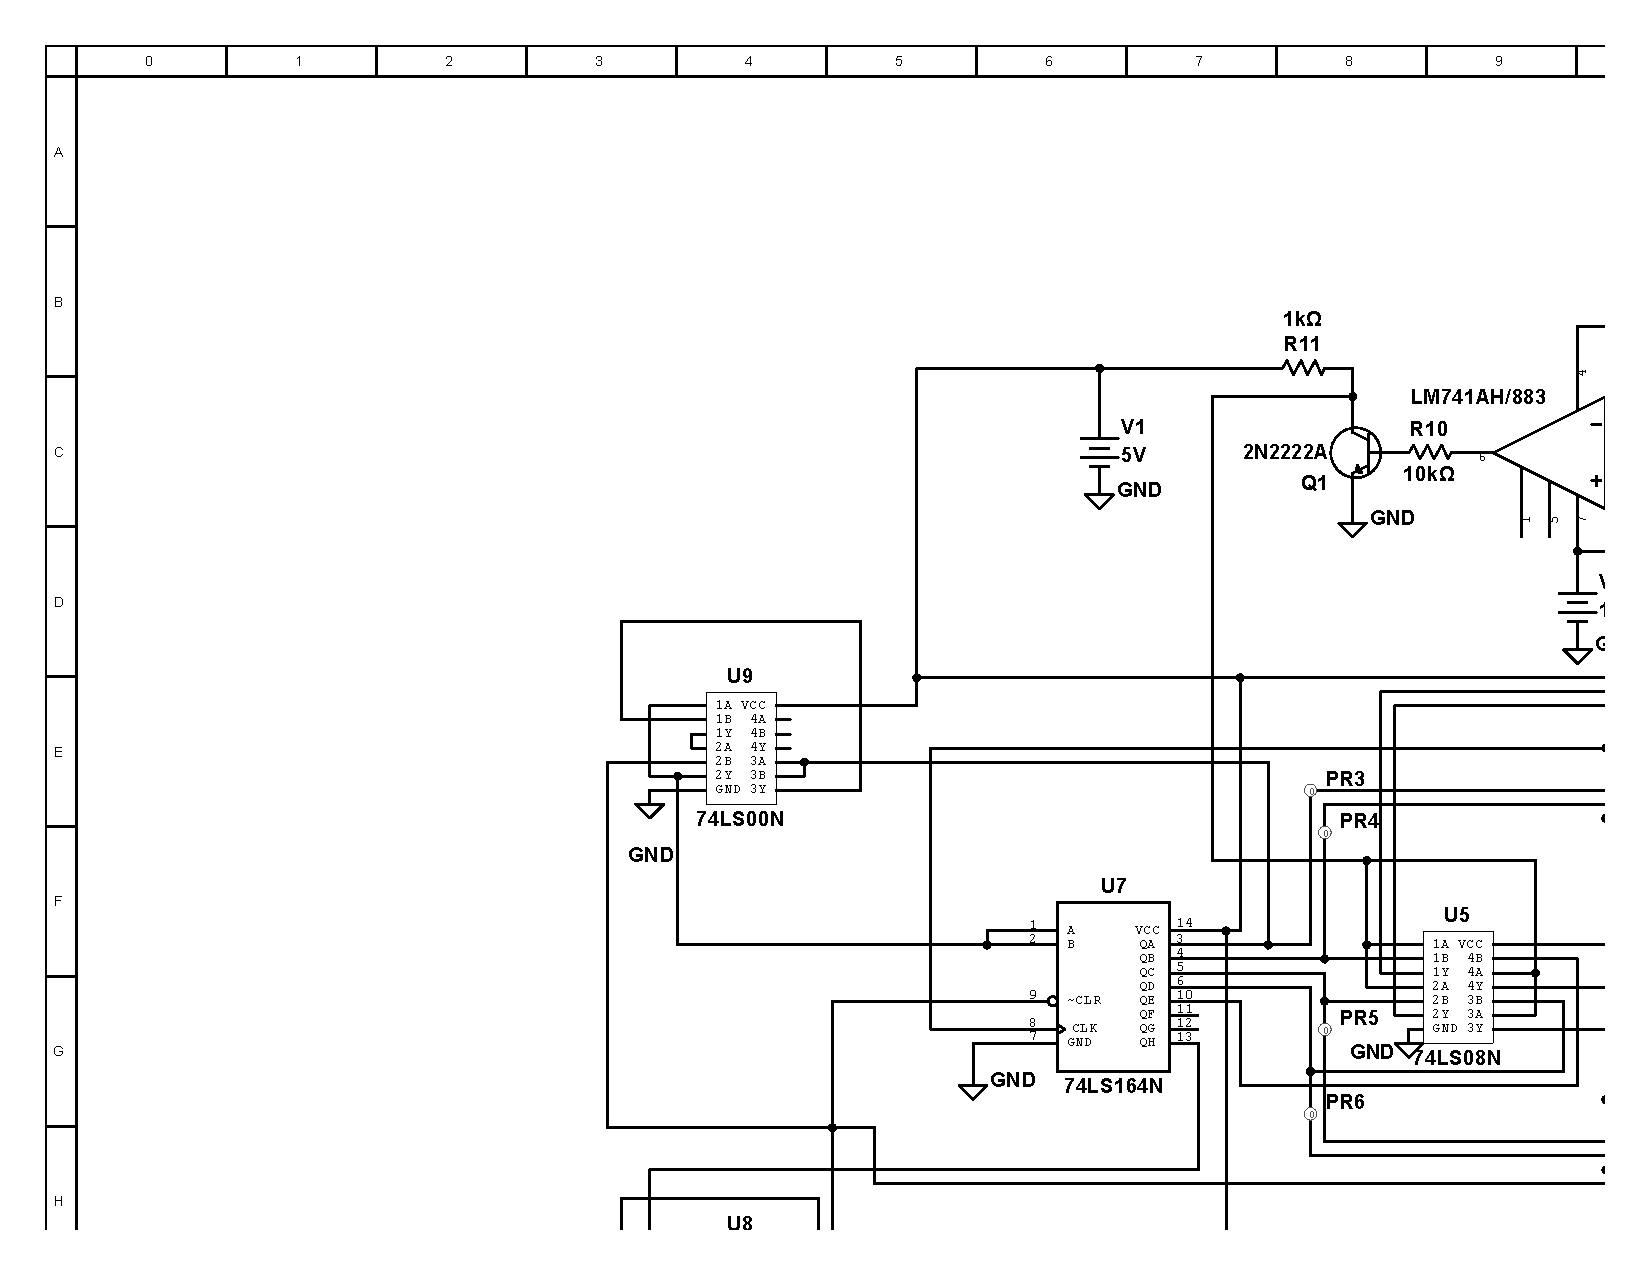
\includegraphics[width=1.15\textwidth]{sch-simulations/output/SAR_4bit_cv1.pdf}
\end{center}
\caption{Schema elettrico completo del convertitore ADC SAR 4 bit}
\label{fig:circuit_sarCompleteSchematic}
\end{figure*}

%%%%%%%%%%%%%%%%%%%%%%%%%%%%%%%%%%%%%%%%%%%%%%%%%%%%%%%%%%%%%
%%%%%%%%%%%%%%%%%%%%%%%%%%%%%%%%%%%%%%%%%%%%%%%%%%%%%%%%%%%%%

\section{Componenti utilizzati}

\subsection{NAND}

\begin{figure}[H]%[!ht]
\begin{center}
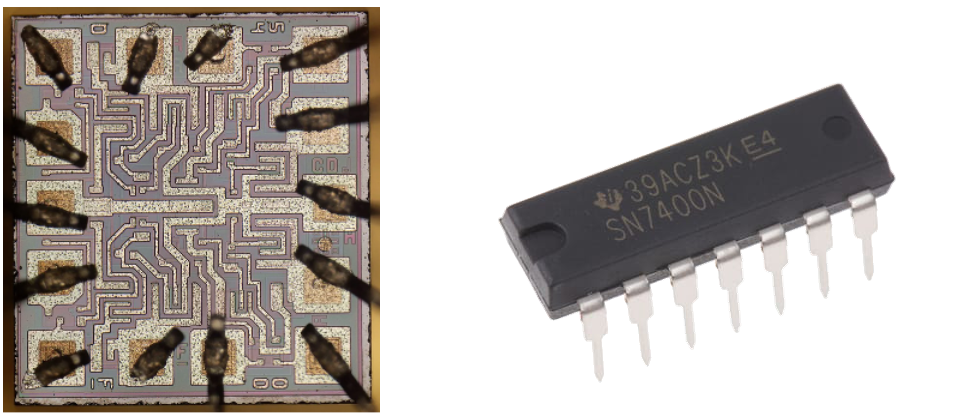
\includegraphics[width=0.40\textwidth]{lab-reports/Schematics-and-graphics/SN7400N.png}
\caption{SN7400N}
\label{fig:integrated_nand}
\end{center}
\end{figure}

\subsection{AND}

\subsection{Transistor}

\subsection{OPA}

\subsection{Resistori}
$R_b = 0.99 \pm 0.01 \ k\Omega$ \\
$R_c = 99 \pm 1 \ k\Omega$








%%%%%%%%%%%%%%%%%%%%%%%%%%%%%%%%%%%%%%%%%%%%%%%%%%%%%%%%%%%%%
%% Primo Giorno 
%%%%%%%%%%%%%%%%%%%%%%%%%%%%%%%%%%%%%%%%%%%%%%%%%%%%%%%%%%%%%

\section{Tabella di verità R-S flip flop}

\begin{figure}[H]%[!ht]
\begin{center}
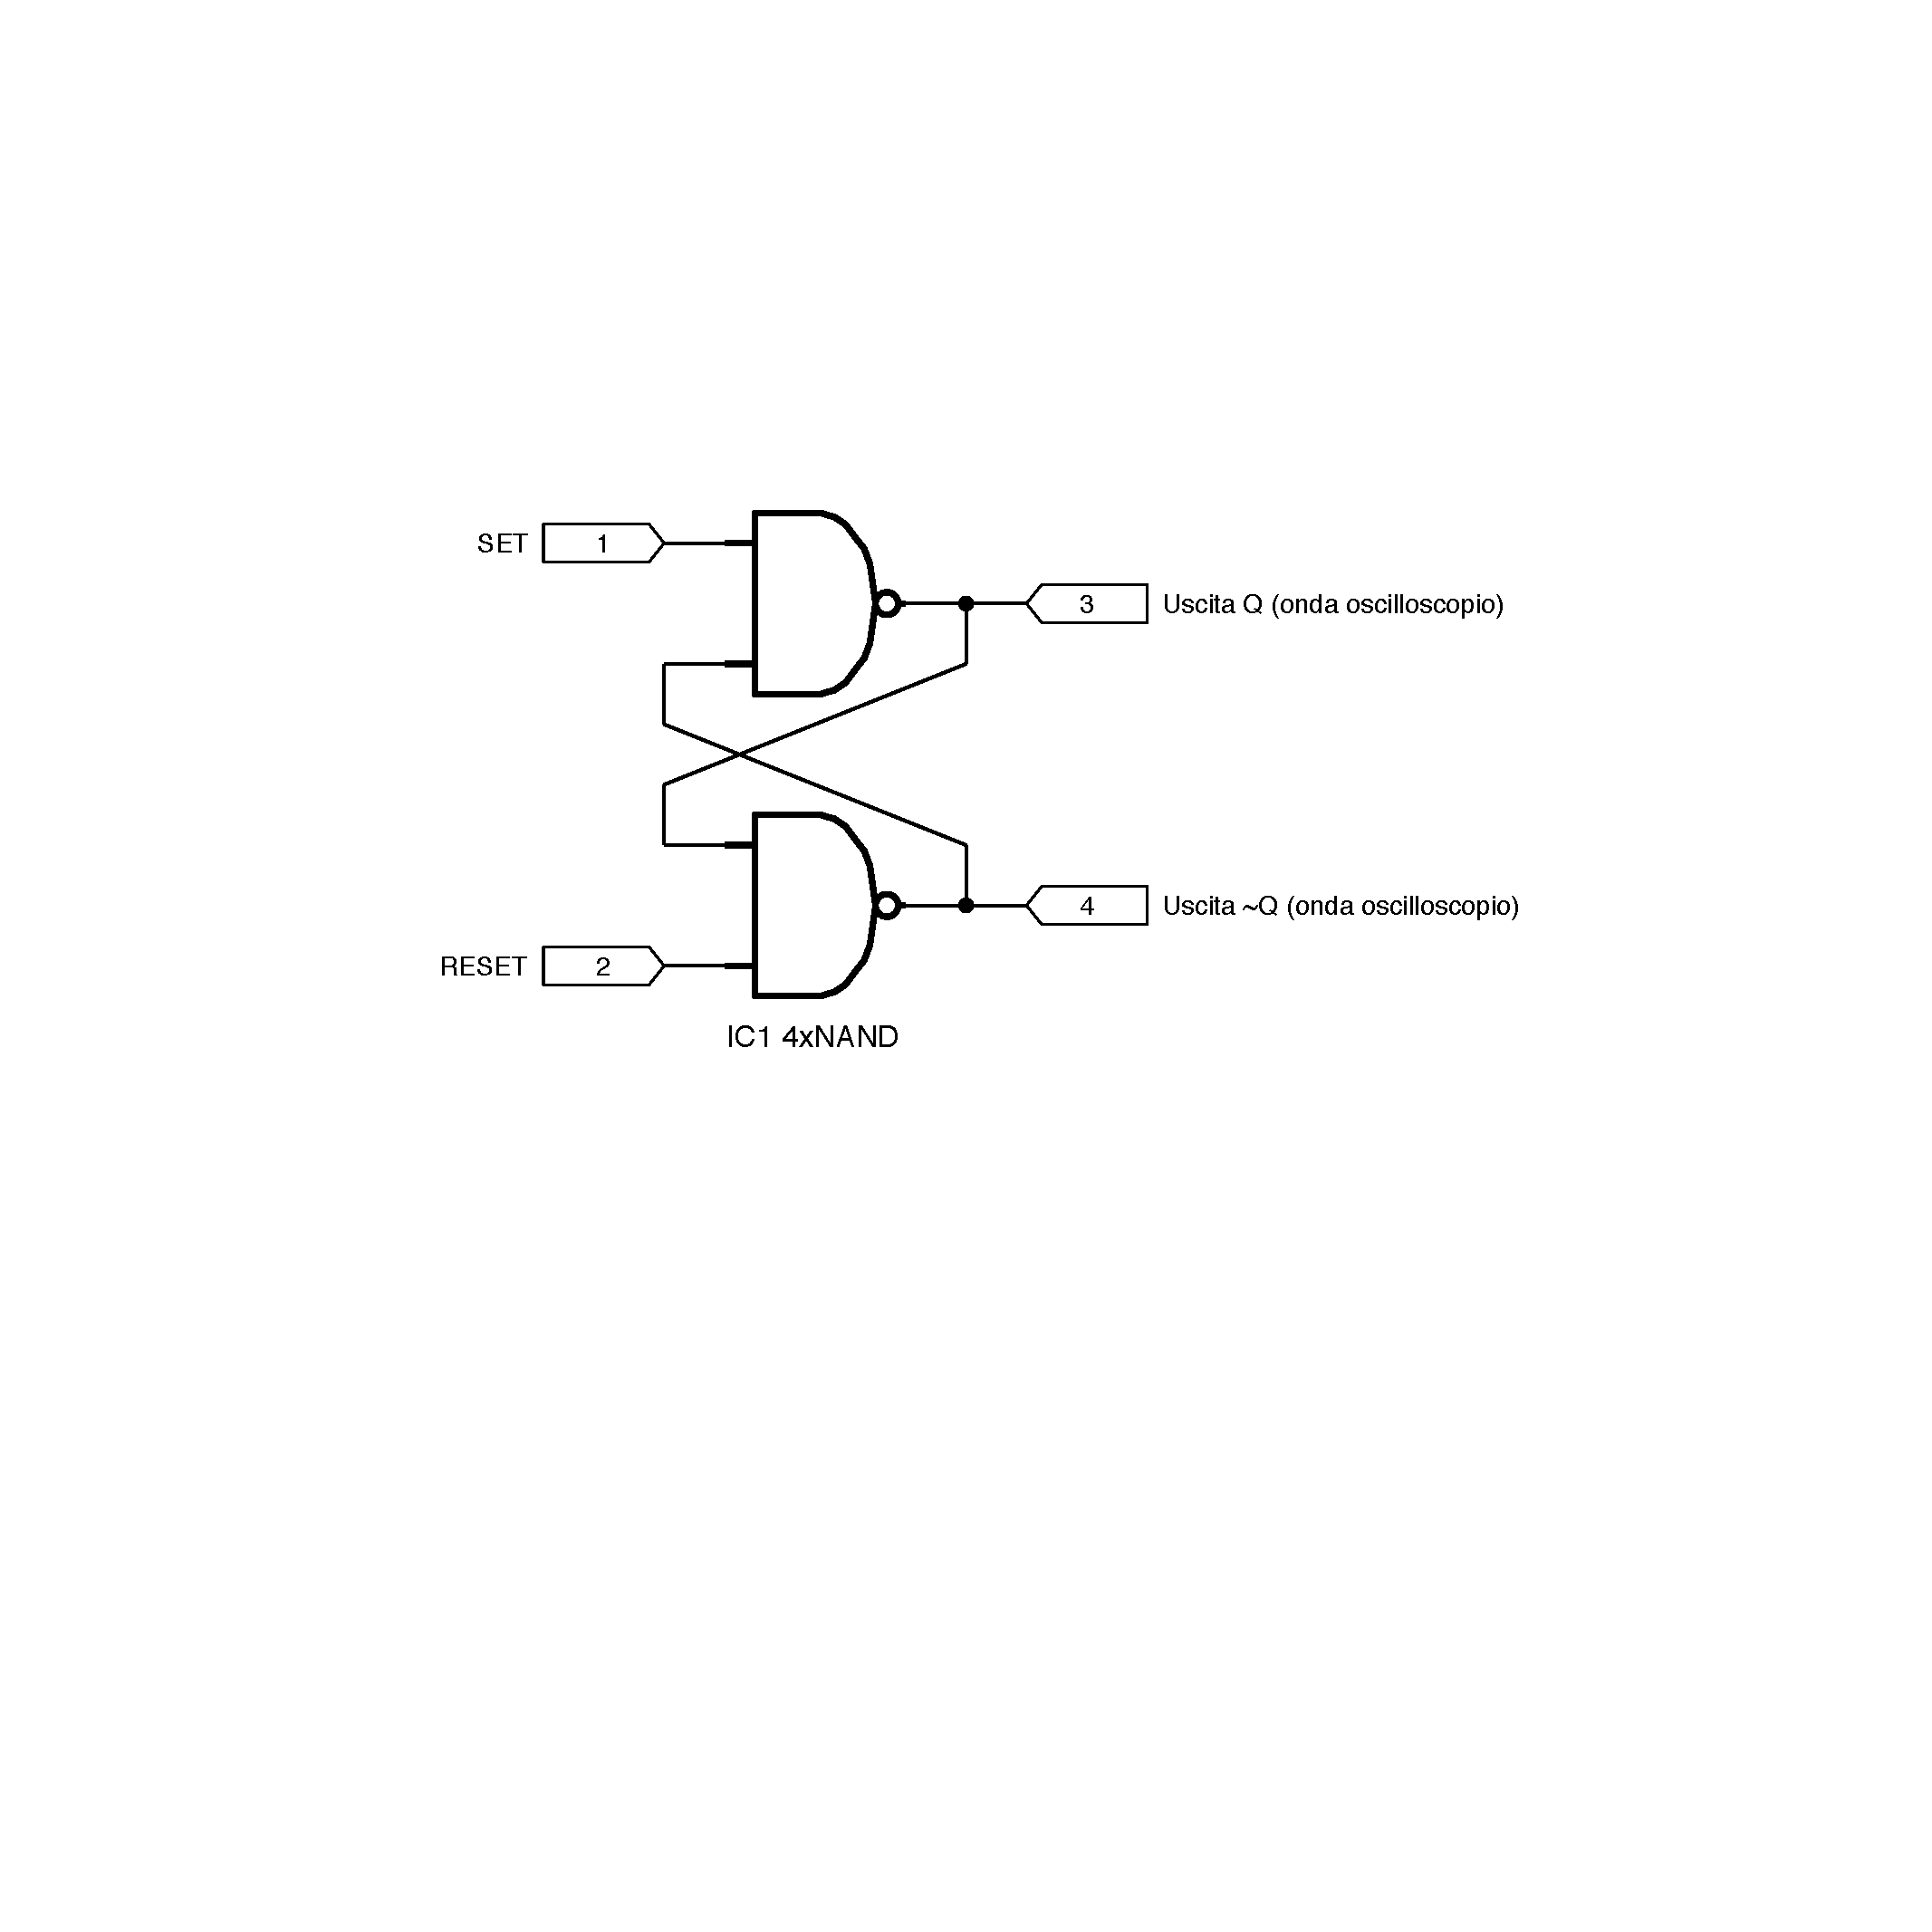
\includegraphics[width=0.40\textwidth]{sch-simulations/digital/output/flip-flop-RS.pdf}
\caption{Flip-flop set - reset}
\label{fig:circuit_flip_flop}
\end{center}
\end{figure}

%%%%%%%%%%%%%%%%%%%%%%%%%%%%%%%%%%%%%%%%%%%%%%%%%%%%%%%%%%%%%

\begin{figure}[H]%[!ht]
\begin{center}
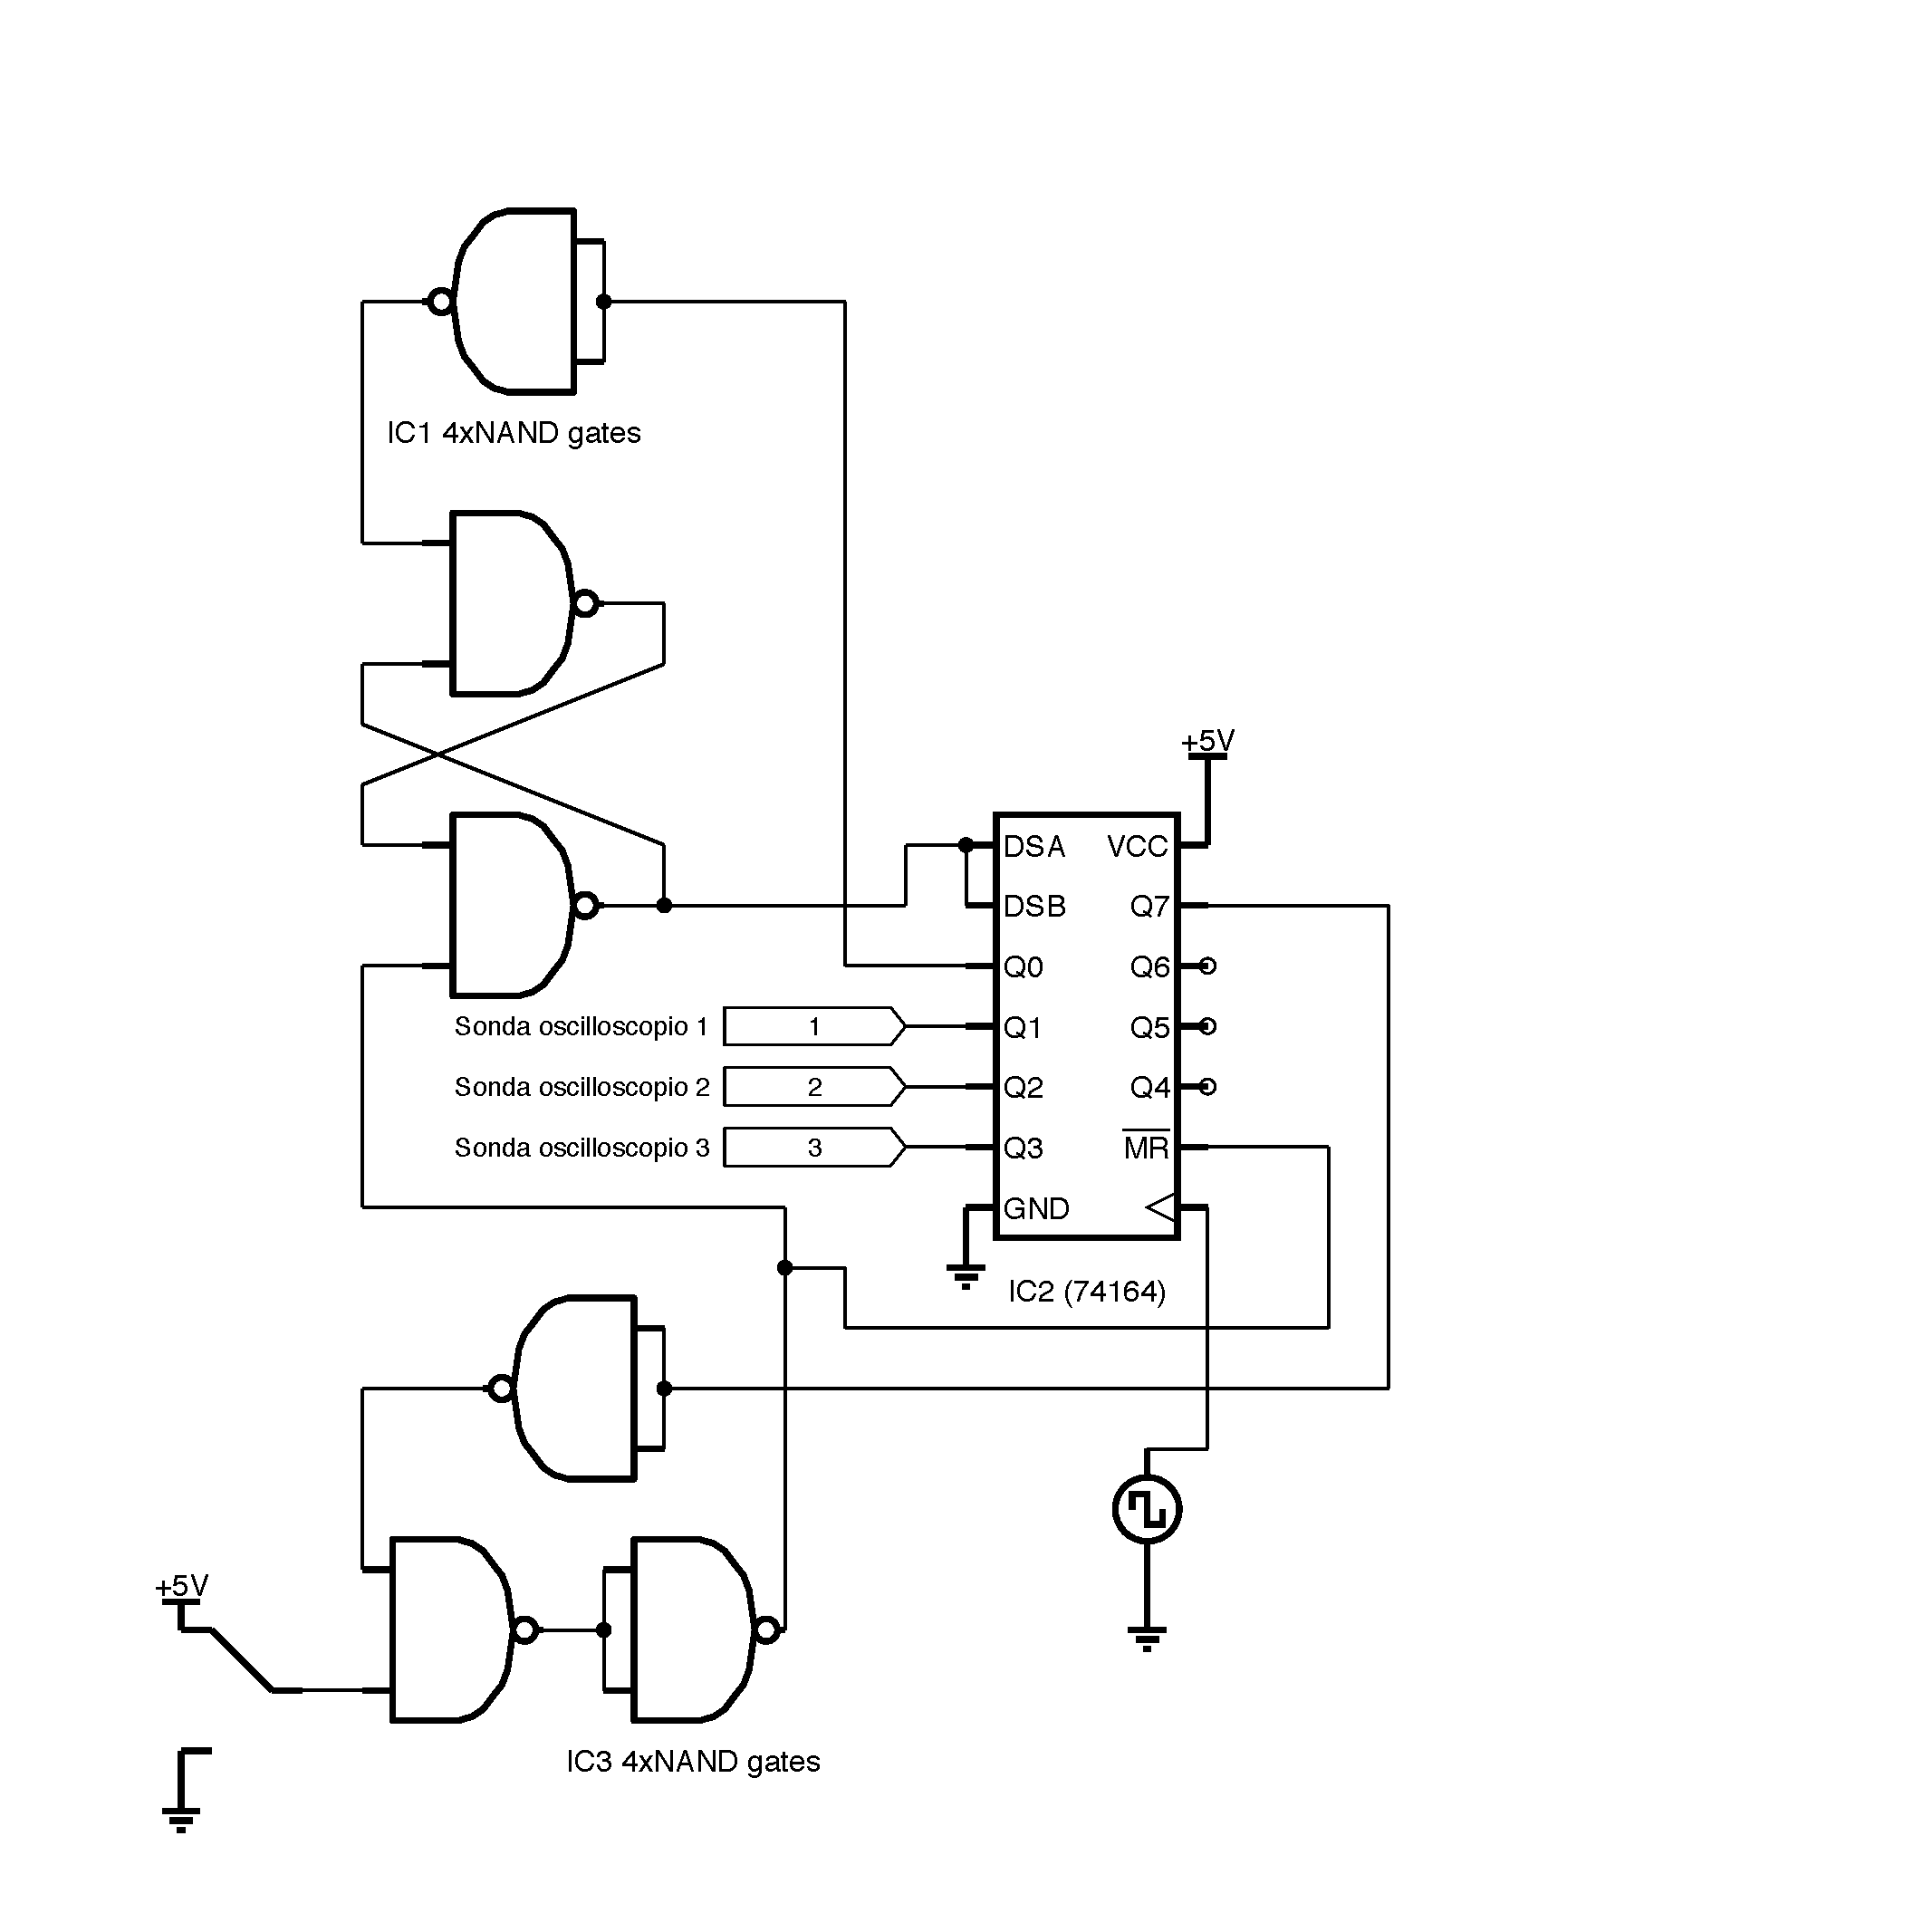
\includegraphics[width=0.54\textwidth]{sch-simulations/digital/output/shift-register.pdf}
\caption{Registro a scorrimento e circuito di controllo}
\label{fig:circuit_shift_register}
\end{center}
\end{figure}


%%%%%%%%%%%%%%%%%%%%%%%%%%%%%%%%%%%%%%%%%%%%%%%%%%%%%%%%%%%%%
%% Secondo Giorno 
%%%%%%%%%%%%%%%%%%%%%%%%%%%%%%%%%%%%%%%%%%%%%%%%%%%%%%%%%%%%%

\section{Tabella di verità AND}

\subsection{Misura $V_{IH}$ }

%%%%%%%%%%%%%%%%%%%%%%%%%%%%%%%%%%%%%%%%%%%%%%%%%%%%%%%%%%%%%

\section{Tabella di verità JK}

%%%%%%%%%%%%%%%%%%%%%%%%%%%%%%%%%%%%%%%%%%%%%%%%%%%%%%%%%%%%%
%% Terzo Giorno 
%%%%%%%%%%%%%%%%%%%%%%%%%%%%%%%%%%%%%%%%%%%%%%%%%%%%%%%%%%%%%


%%%%%%%%%%%%%%%%%%%%%%%%%%%%%%%%%%%%%%%%%%%%%%%%%%%%%%%%%%%%%
%% Appendice
%%%%%%%%%%%%%%%%%%%%%%%%%%%%%%%%%%%%%%%%%%%%%%%%%%%%%%%%%%%%%


\begin{appendices}

\section{Oscillatore ad anello}

\begin{figure}[H]%[!ht]
\begin{center}
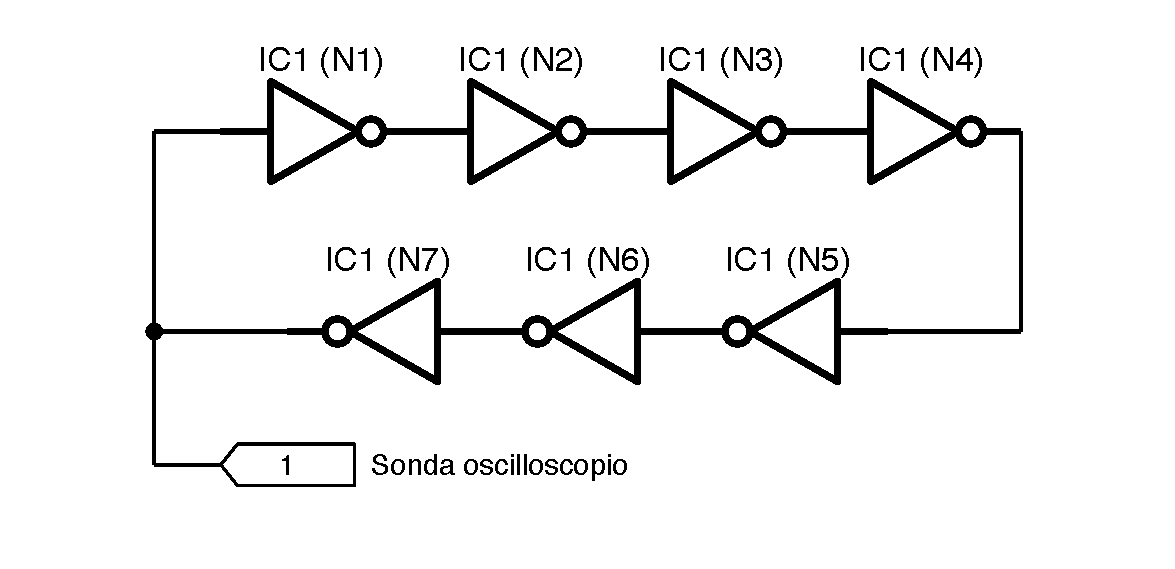
\includegraphics[width=0.40\textwidth]{sch-simulations/digital/output/ring-osc-logic.pdf}
\caption{Circuito equivalente dell'oscillatore ad anello}
\label{fig:circuit_ring_oscillator}
\end{center}
\end{figure}

\begin{figure}[H]%[!ht]
\begin{center}
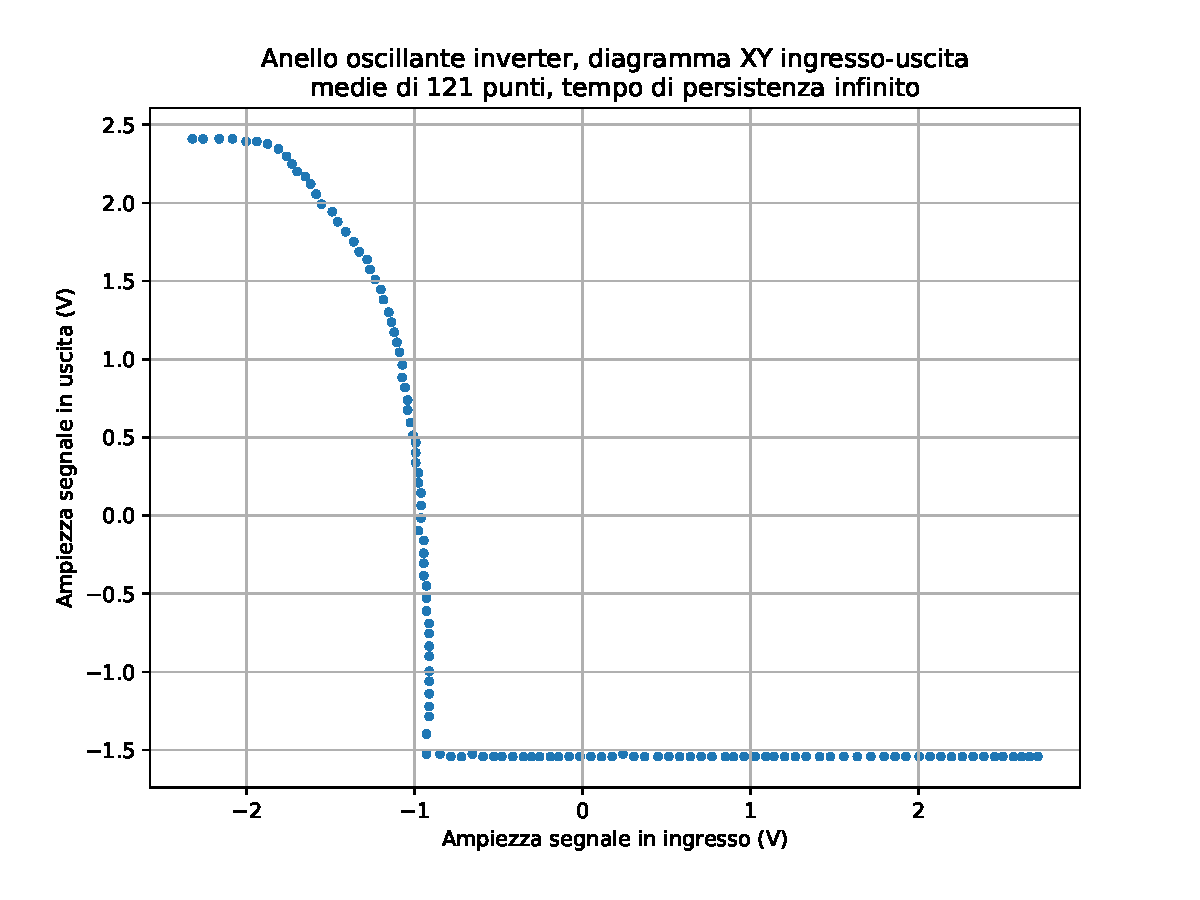
\includegraphics[width=0.48\textwidth]{analysis/output/inverter_ring_xy.pdf}
\caption{Studio dell'oscillatore ad anello}
\label{fig:inverter_ring_xy}
\end{center}
\end{figure}

%%%%%%%%%%%%%%%%%%%%%%%%%%%%%%%%%%%%%%%%%%%%%%%%%%%%%%%%%%%%%

\section{Caratterizzazione transistor npn}


\end{appendices}

%%%%%%%%%%%%%%%%%%%%%%%%%%%%%%%%%%%%%%%%%%%%%%%%%%%%%%%%%%%%%
%% Indice e Bibliografia 
%%%%%%%%%%%%%%%%%%%%%%%%%%%%%%%%%%%%%%%%%%%%%%%%%%%%%%%%%%%%%

\clearpage
\newpage

\tableofcontents % Indice

\printbibliography % Bibliografia

\end{document}